\documentclass[]{scrartcl}
\usepackage{Preamble}

\renewcommand{\exercise}{Exercise 2}
\renewcommand{\duedate}{2020-06-08, 18:00}

\begin{document}
\section{Buffer}
\subsection{Auslastung von line}
Bei der Simulation des Netzwerks \"uber \SI{200}{\micro\second} f\"allt auf,
dass in etwas mehr als der H\"alfte der F\"alle das Senden die Queue \"andert.
Der Puffer wird also genutzt. Unter Betrachtung der mittleren Puffertiefe in 
Abbildung~\ref{fig:buffer_depth} k\"onnen
wir aber sagen, dass der Kanal nicht \"uberlastet wird da diese im Mittel 1 und
im Maximum 7 betr\"agt.
\begin{figure}[ht]
    \centering
    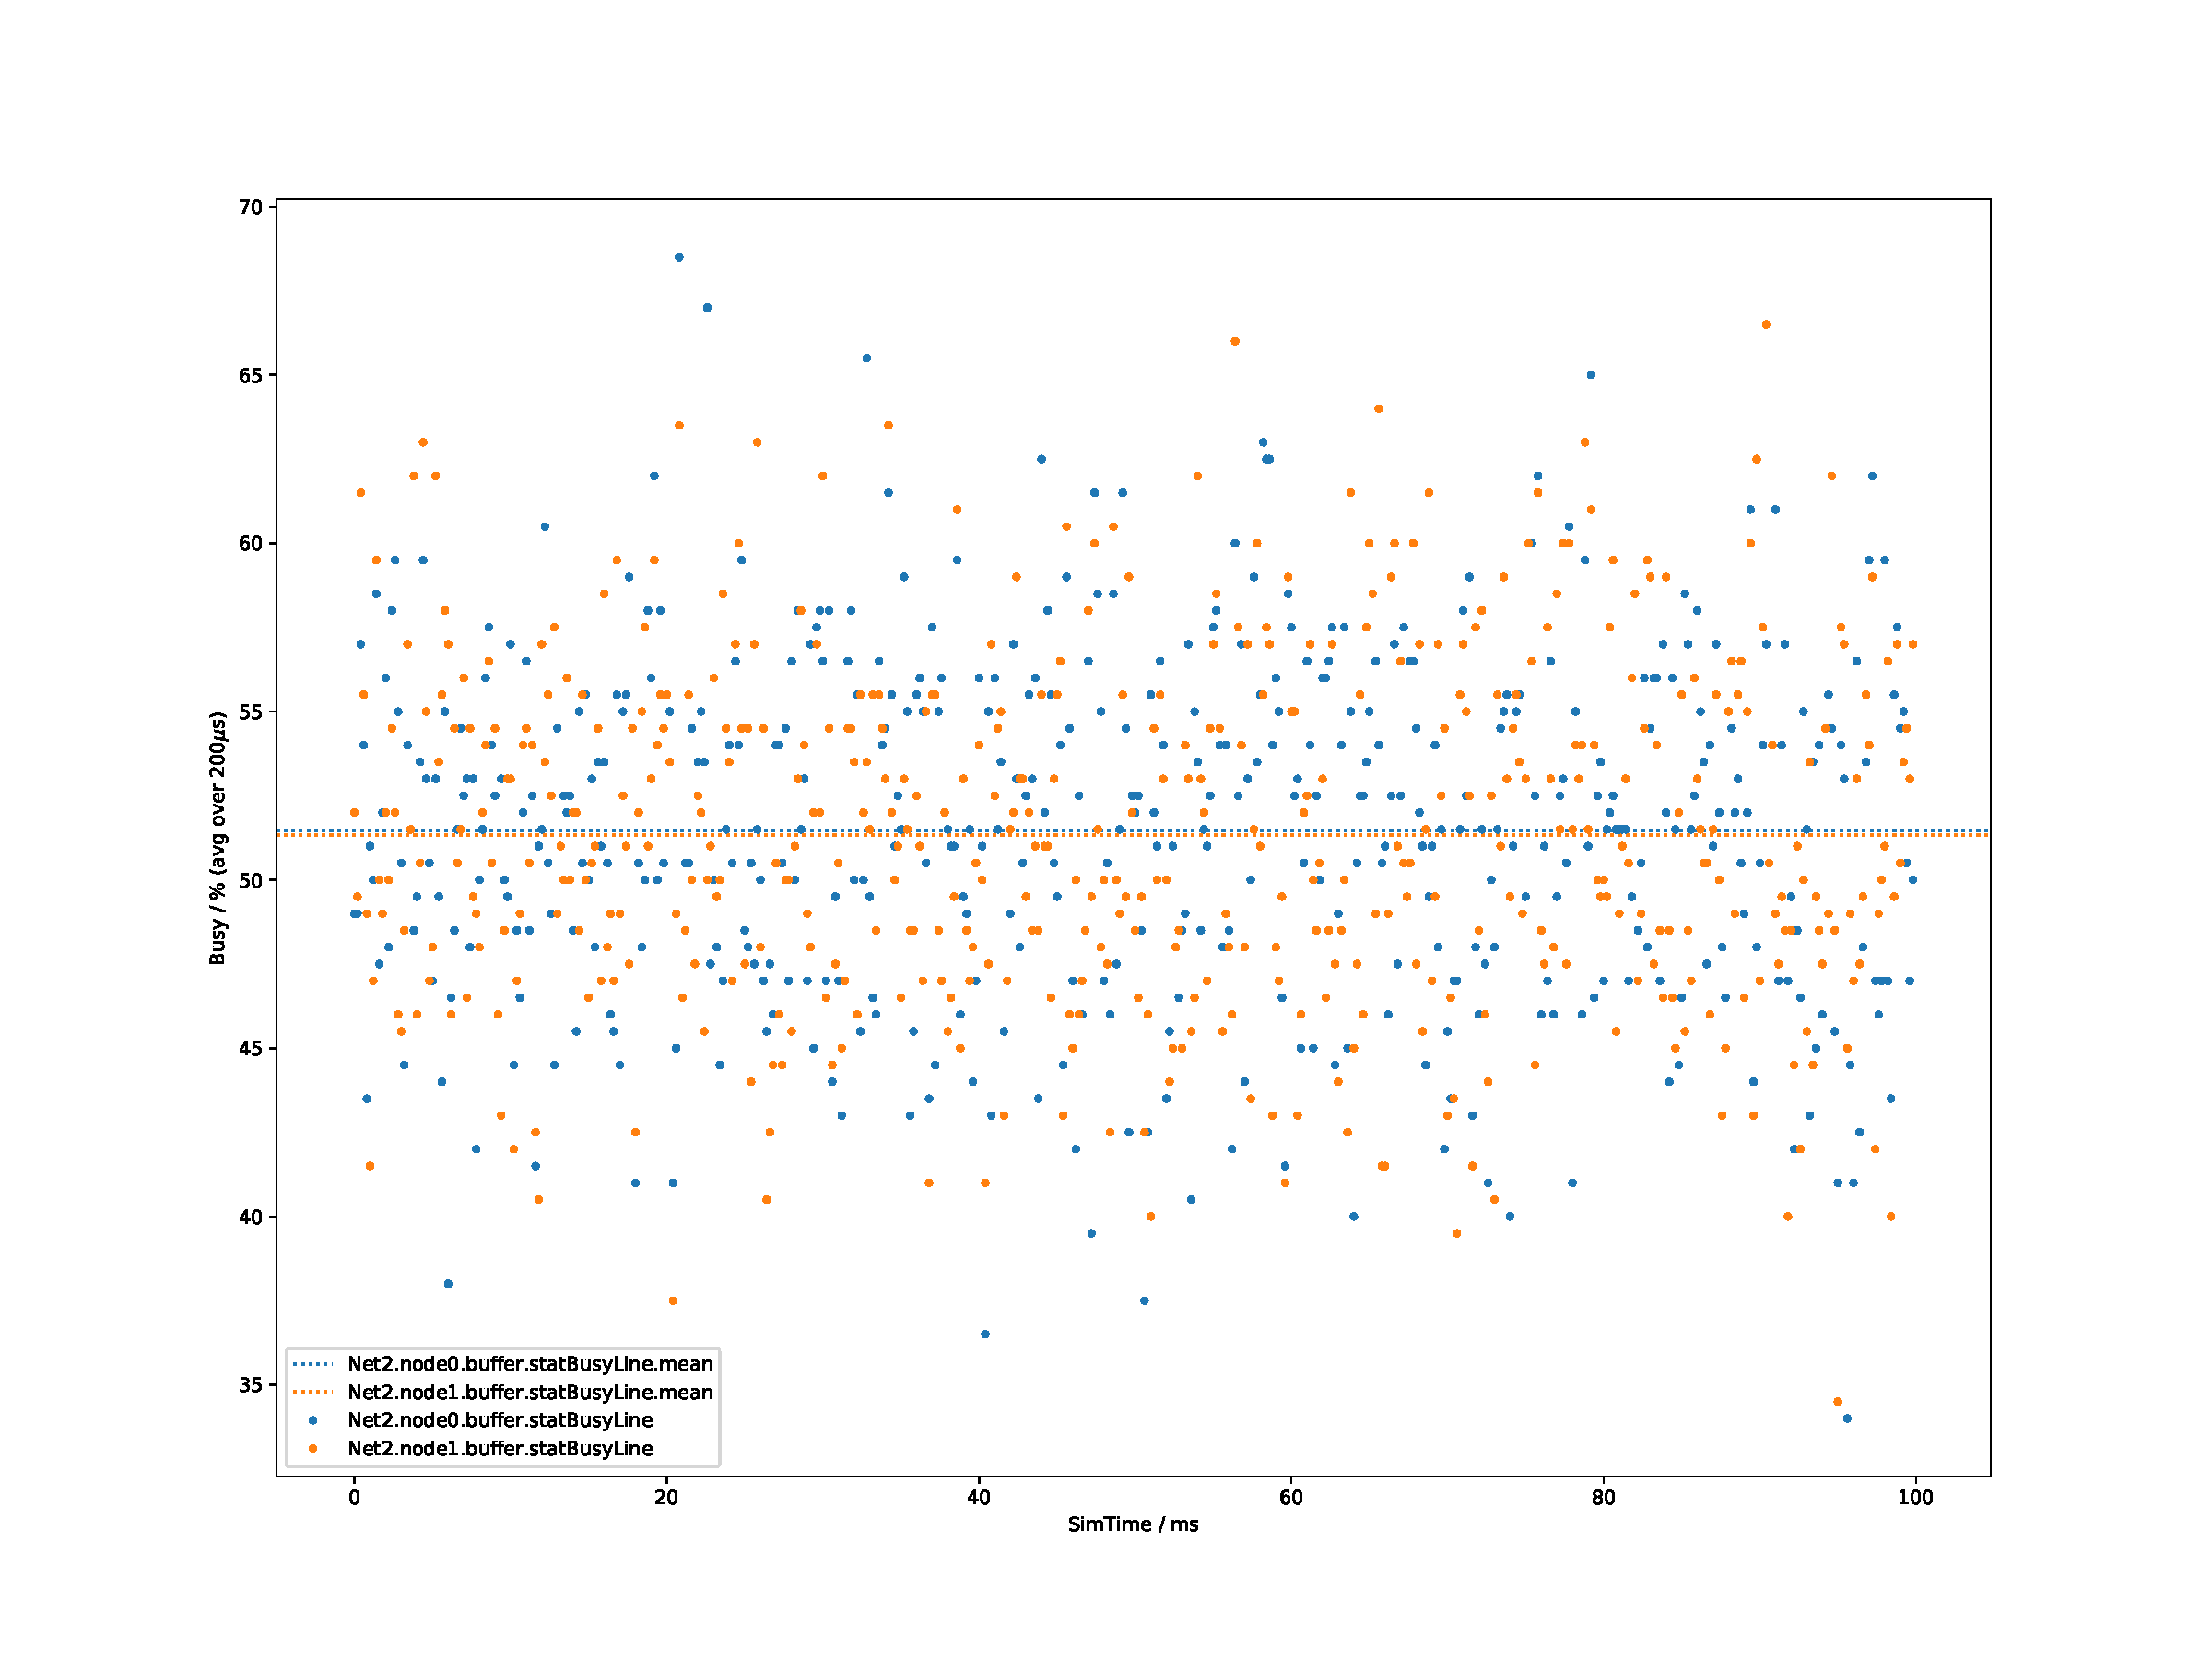
\includegraphics[width=\columnwidth]{../../python/03_01.pdf}
    \caption{Auslastung von line, bei einer Abfragefrequenz von \SI{1}{GHz} und der Mittelung von 200 Abfragen}
\end{figure}
\newpage
\subsection{Number of Packets waiting in Queue}

\begin{figure}[ht]
    \centering
    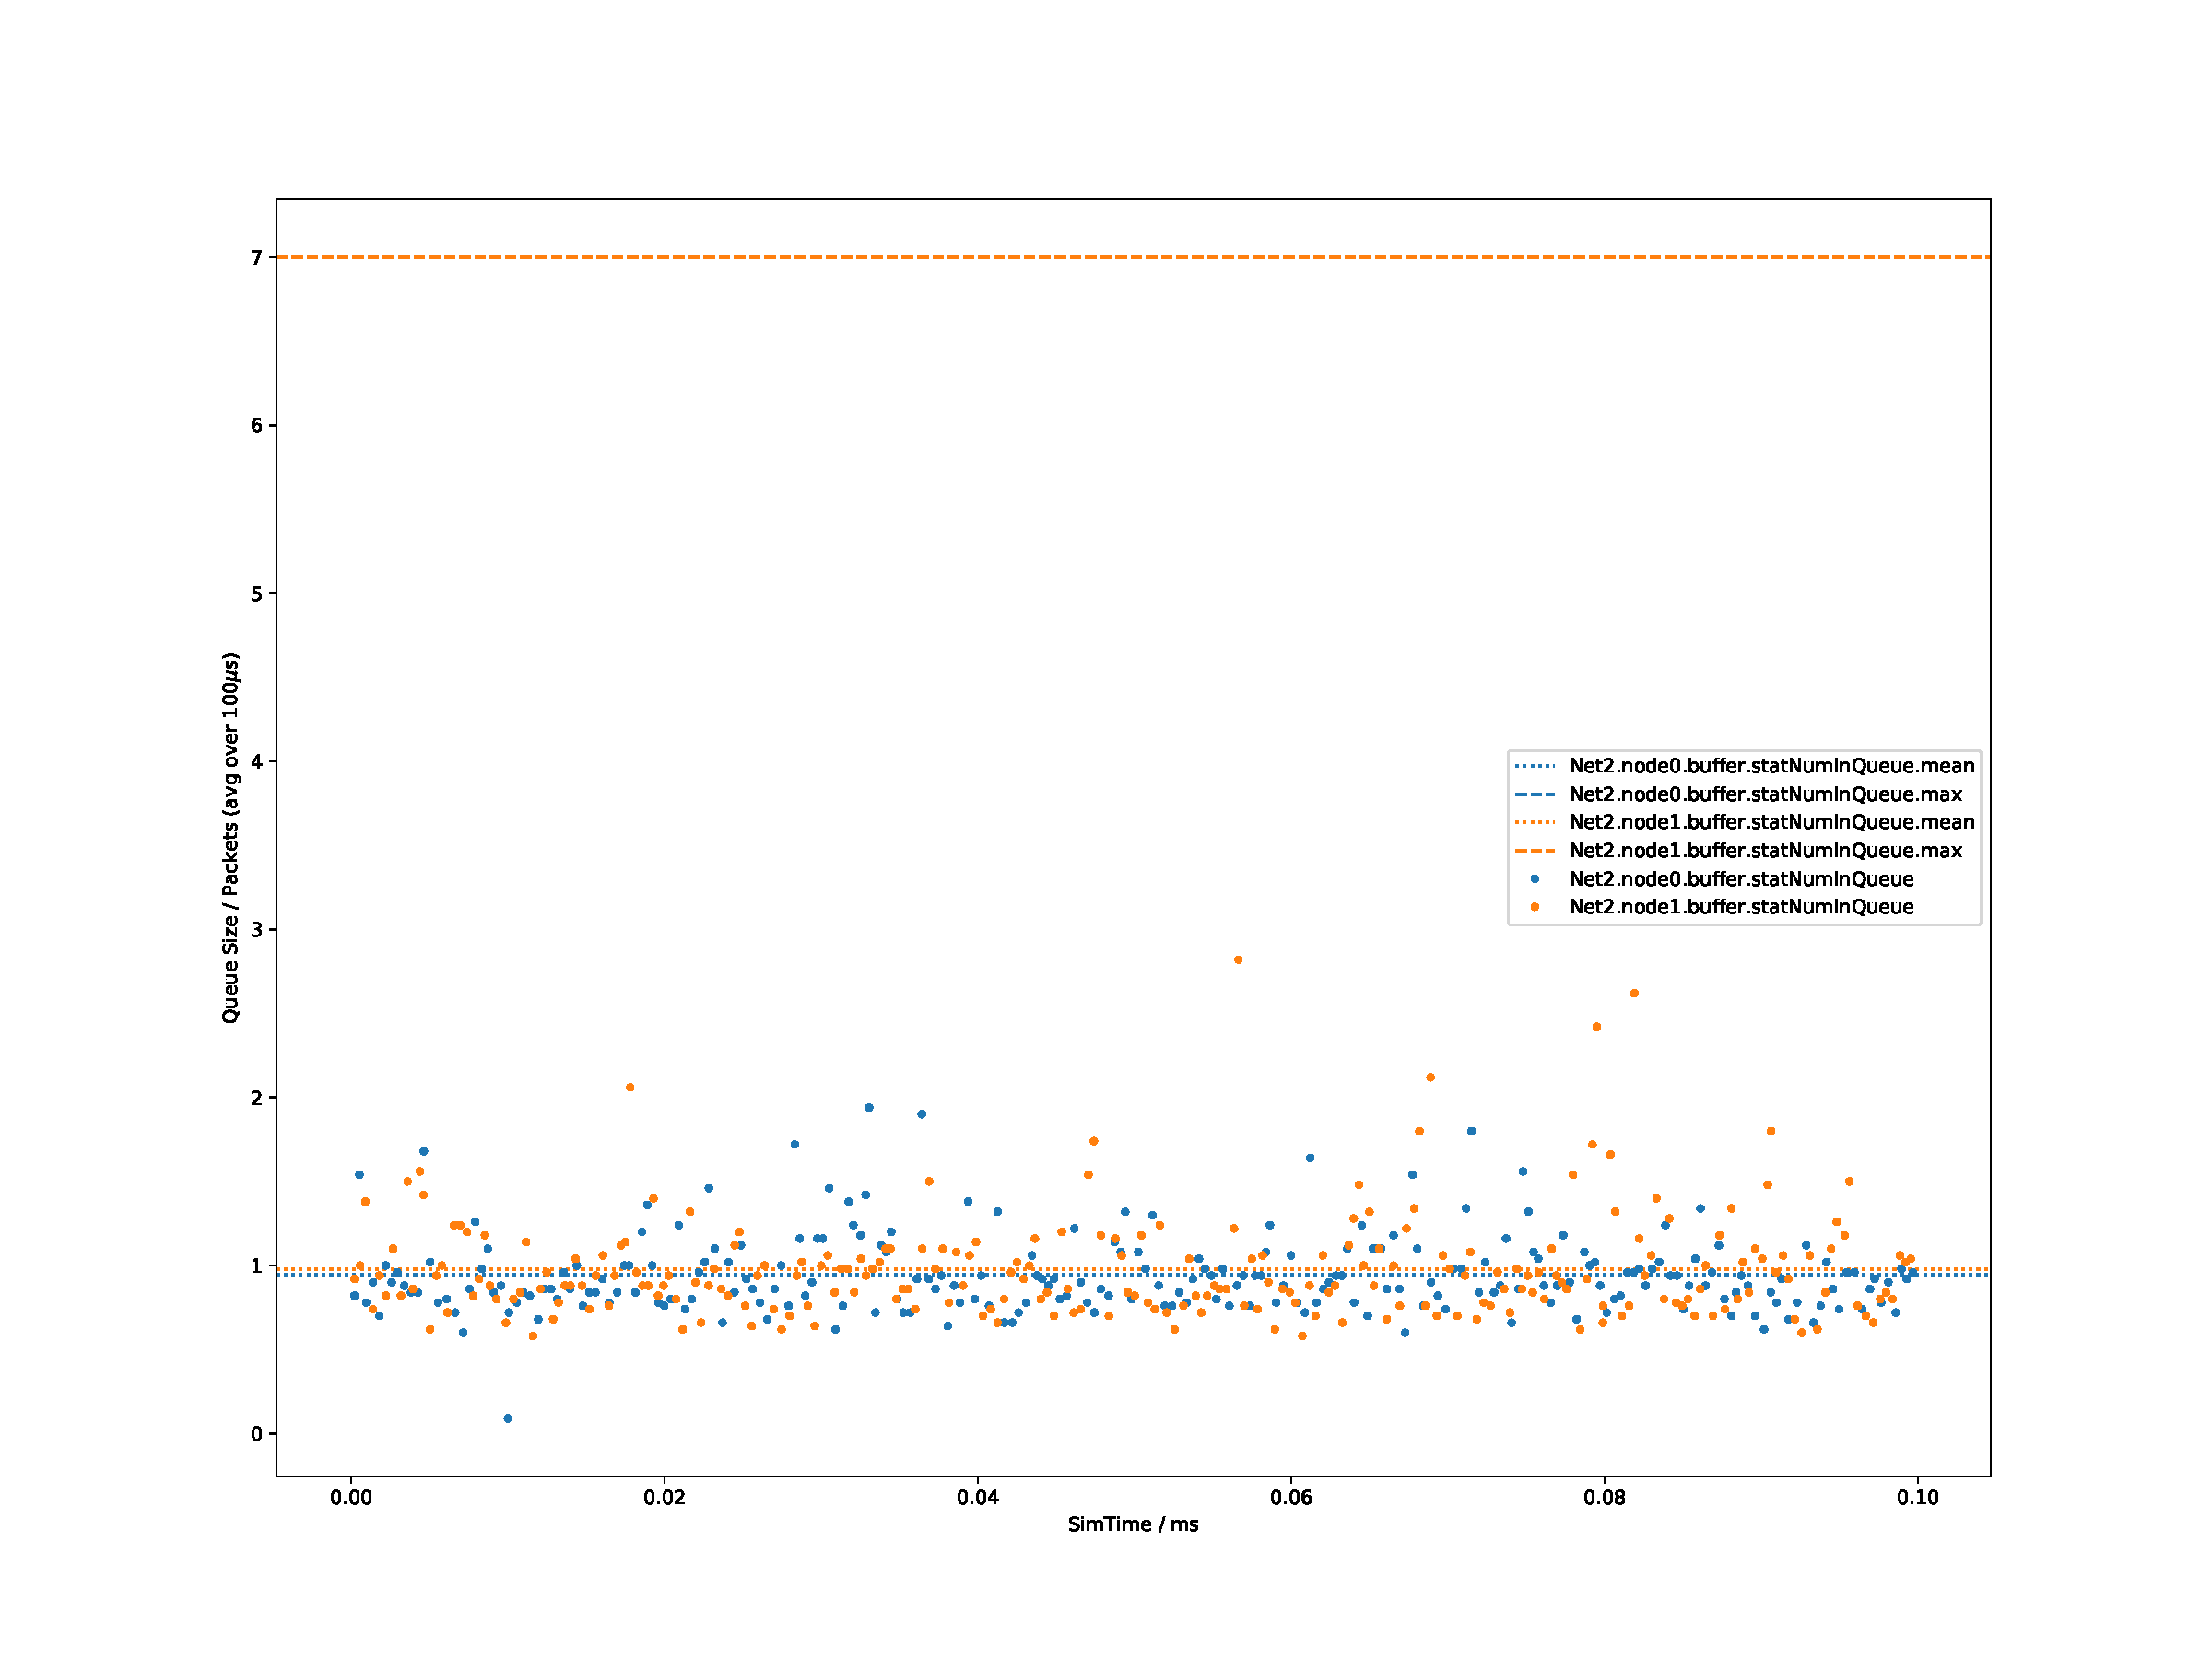
\includegraphics[width=\columnwidth]{../../python/03_02.pdf}
    \caption{}
    \label{fig:buffer_depth}
\end{figure}
\end{document}
